% LINEAR SYSTEMS AND CONTROL
% Homework 5 : 

\documentclass[10pt,a4paper]{article}
\usepackage[latin1]{inputenc}
\usepackage{amsmath}
\usepackage{amsfonts}
\usepackage{amssymb}
\usepackage{graphics} 
\usepackage{graphicx}
\usepackage{float}
\usepackage{subfigure}
\usepackage{mathtools}

\usepackage{trfsigns}
\author{Ana Huaman}
\title{\textbf{Homework 5} \\ ECE 6550: Linear Control and Systems}
\date{}
\begin{document}
\maketitle

%%%%%%%%%%%%%%%%%%%%%%%%%%%%%%%%%%%%%%%%%
% Question 1
%%%%%%%%%%%%%%%%%%%%%%%%%%%%%%%%%%%%%%%%%
\section{}
Go to T-Square under Resources/m-file and download the m-file dist.m. This is a model of a distillation process

\subsection*{a}
Is this system completely controllable? Is the uncontrolled system stable?

\subsection*{Solution}
Our system has $n=5$, so no way I am doing this by hand. Let's use Octave (Matlab's free sister). 

\begin{itemize}
\item{ \textit{Stability:} We find the eigenvalues of $A$:
\[ eig(A) = \{-24.1755, -16.4722, -5.4012, 20.0907, 15.3074 \} \]
The last $2$ eigenvalues are on the right side of the plane, so:
\begin{center}
\fbox{The system is not stable}
\end{center} }

\item{ \textit{Controllability:} We find the controllability matrix ($\Gamma_{5 \times 10}$) and its rank:
\[ rank(\Gamma) = 5 \]
Since the rank is the same as $n = 5$
\begin{center}
\fbox{The system is Completely controllable}
\end{center} }
\end{itemize}

\subsection*{b}
By picking weights, come up with a controller that makes the system behave "well" (This is vague - just like life as a control designer is...)

\subsection*{Solution}
First, let's see how the system behaves with the default values ( $R = I$ and $Q = I$ ). Here the plots:

	\begin{figure}[H]
			\centering
			  \subfigure[$x(t)$ vs $t$]{
			  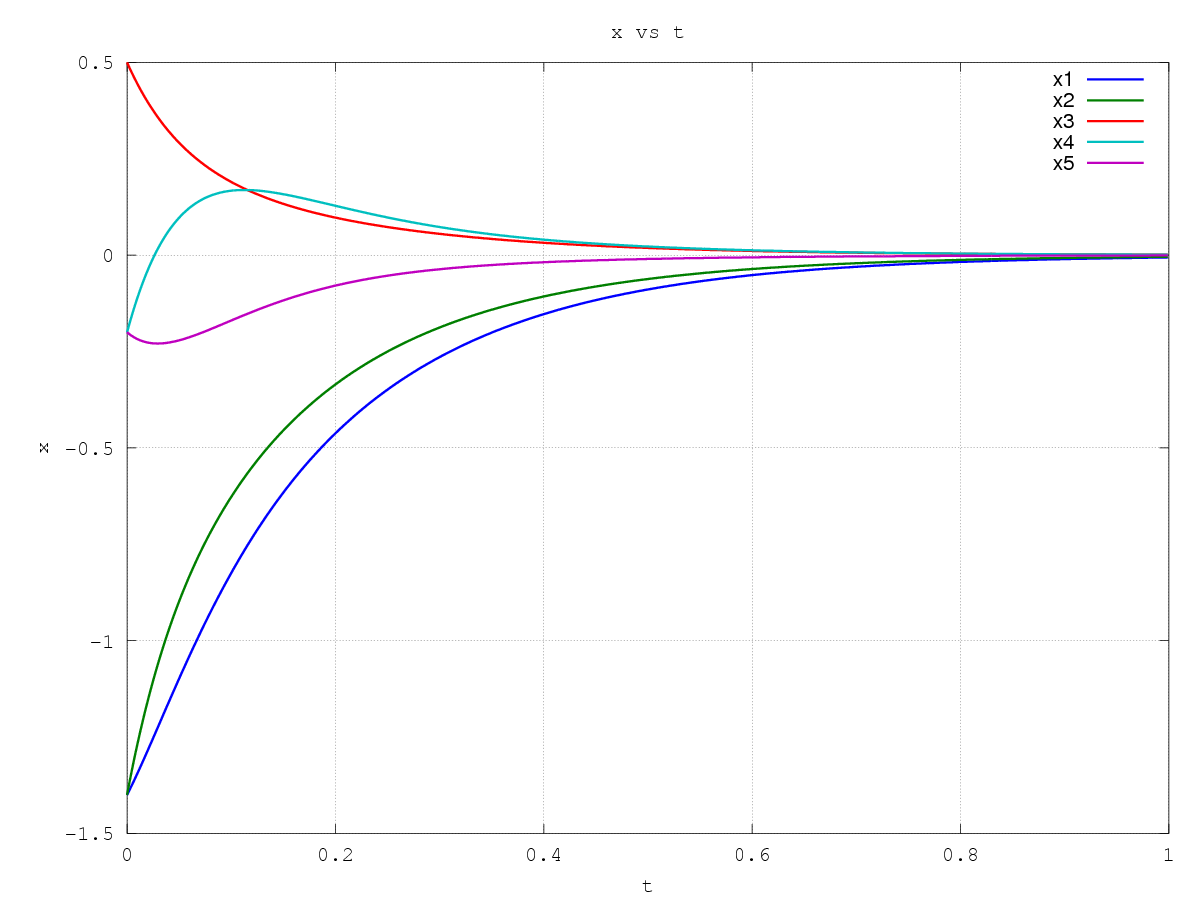
\includegraphics[scale=0.275]{figures/Question1x0.png} 
	          \label{fig:Q1-x0}
              }
              \subfigure[$u(t)$ vs $t$]{
	          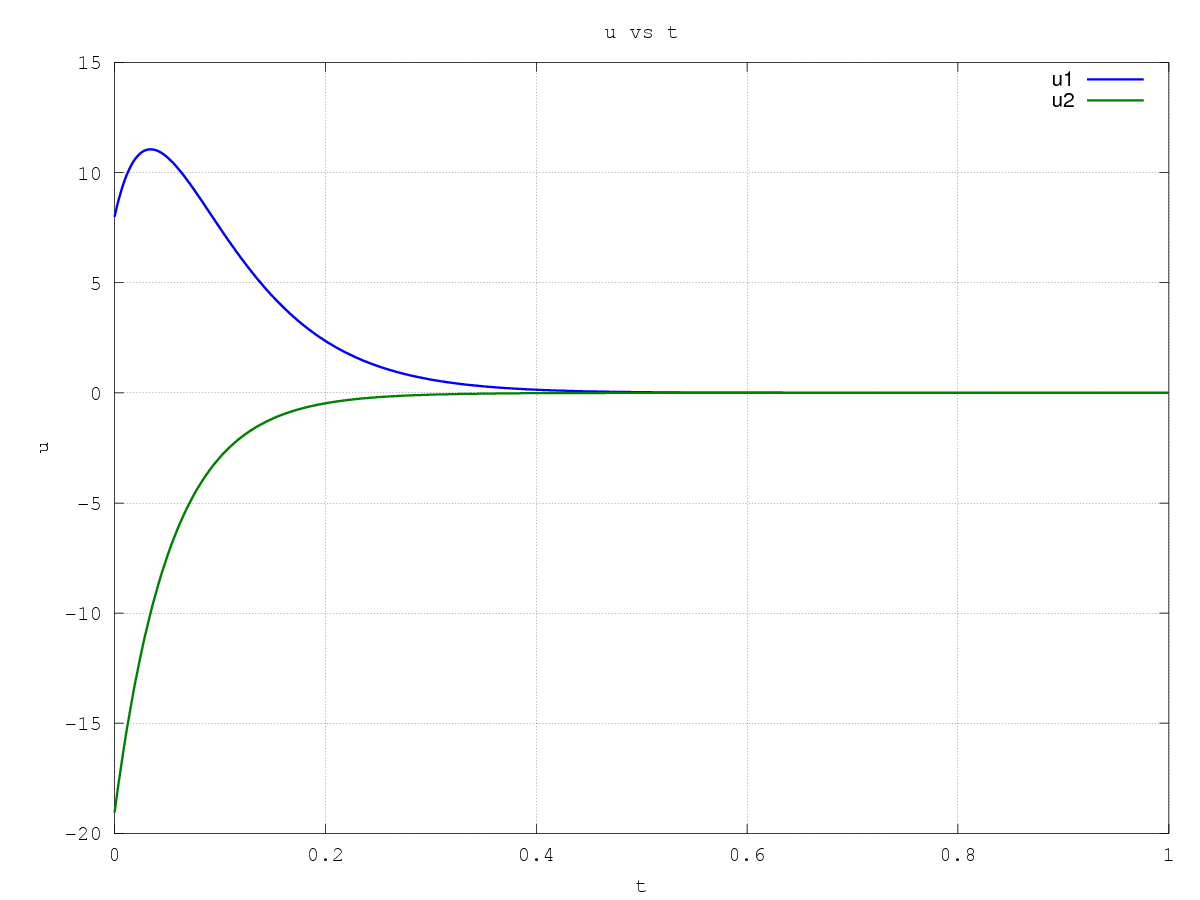
\includegraphics[scale=0.275]{figures/Question1u0.png} 	
	          \label{fig:Q1-u0}
              }
            \caption{Results with $R = I$ and $Q = I$}
            \label{fig:Q1-xu0}
	\end{figure}

The first thing that catch my eye is that $u_{1}$ value jumps at the beginning, so let's solve that. I did some trials to update $R$ such that the cost for $u_{1}$ is higher with respect to $u_{2}$. I got a "good" result with $u_1$ cost being 5 times higher than the cost for $u_{2}$, meaning:

\[
R = \begin{bmatrix}
5 & 0 \\
0 & 1
\end{bmatrix} 
\]

We get the following plots:

	\begin{figure}[H]
			\centering
			  \subfigure[$x(t)$ vs $t$]{
			  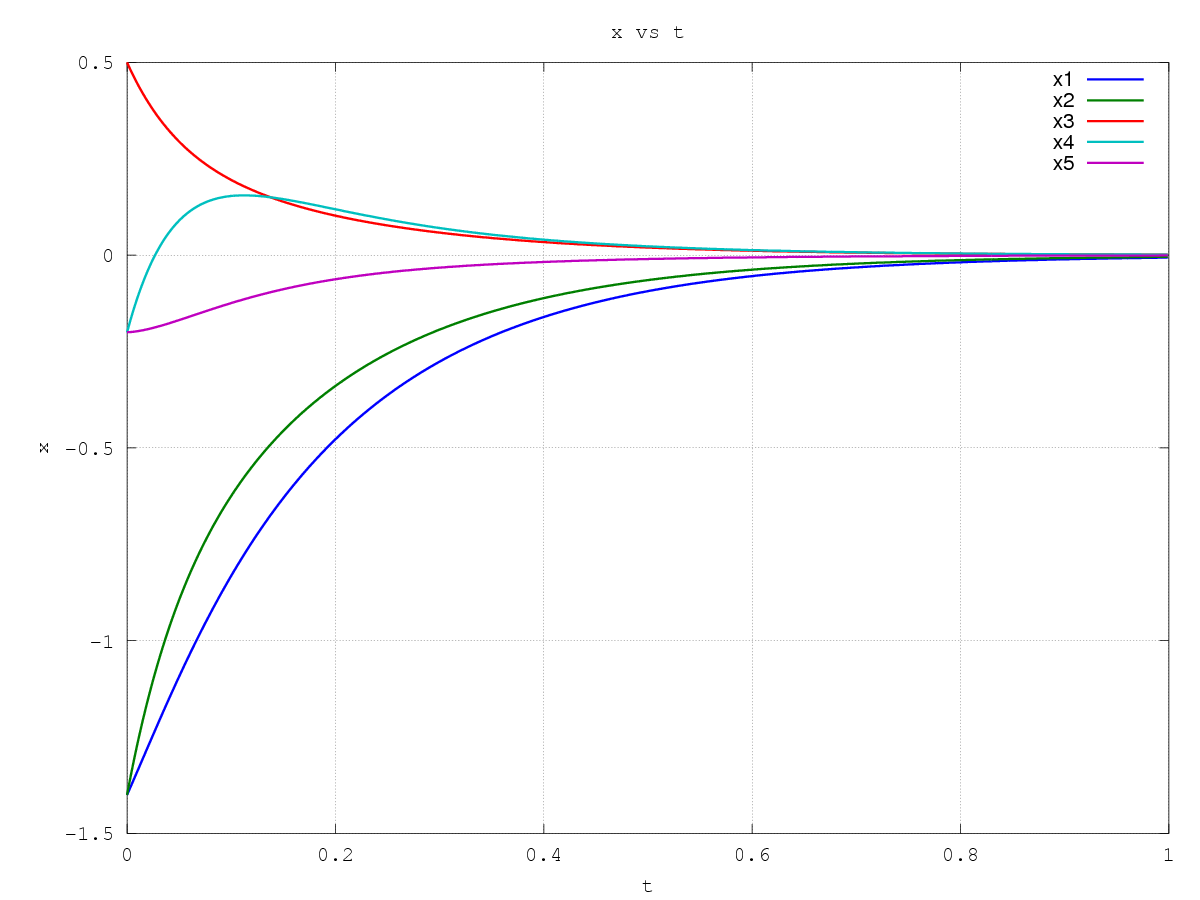
\includegraphics[scale=0.275]{figures/Question1x1.png} 
	          \label{fig:Q1-x1}
              }
              \subfigure[$u(t)$ vs $t$]{
	          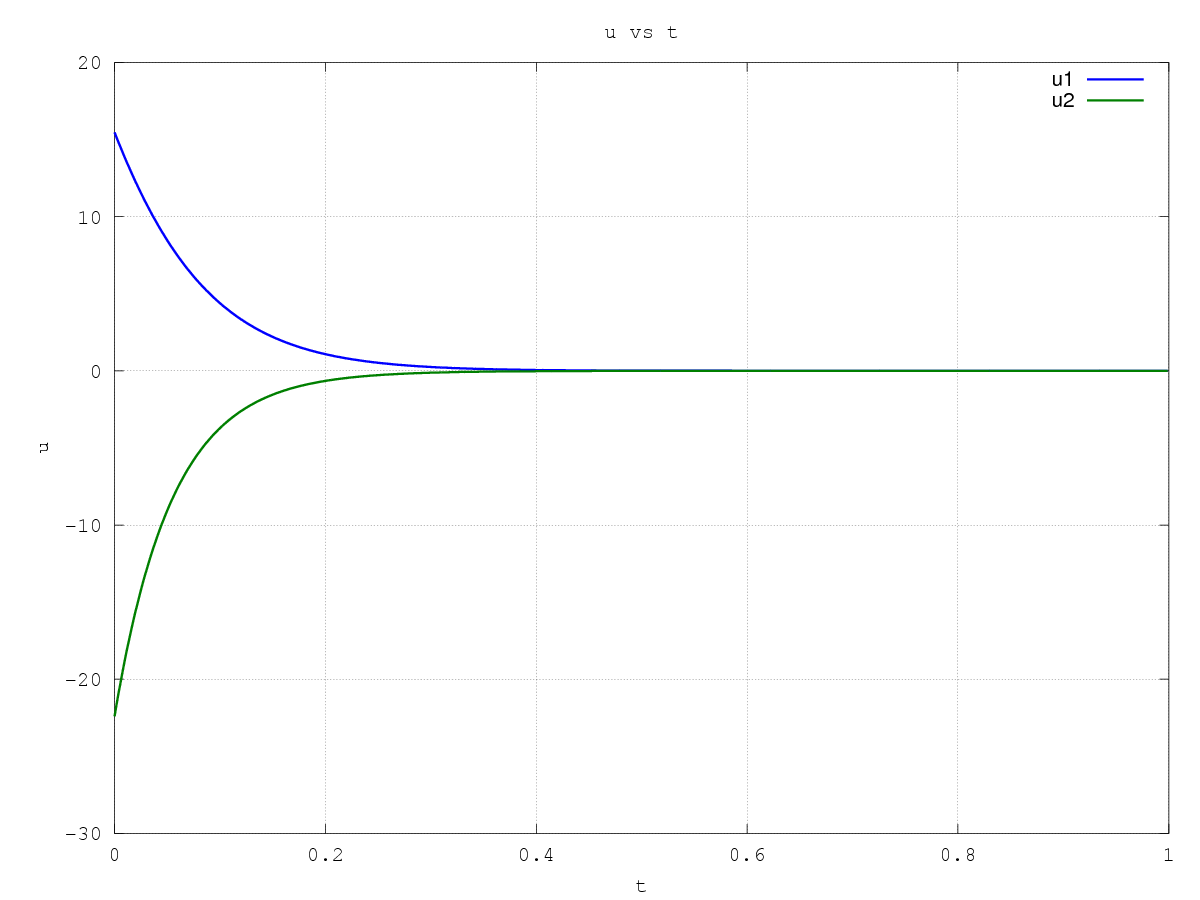
\includegraphics[scale=0.275]{figures/Question1u1.png} 	
	          \label{fig:Q1-u1}
              }
            \caption{Results with $R$ such that $R(1,1) = 5$, $R(2,2) = 1$ and $Q = I$}
            \label{fig:Q1-xu1}
	\end{figure}

Now $u_{1}$ looks good! It goes smoothly down and the bump is gone. Yay.
\medskip

Next I wanted to make the states $x$ go quicker to zero by making $Q$ bigger, however I did not observed any significant improvement. Also, I tried to give more weight to $x_{4}$ since it has also a small bump at the beginning of the process, but again, I did not find any particular improvement in the plots. So, I settled with these values:

\[
R = \begin{bmatrix}
5 & 0 \\
0 & 1
\end{bmatrix} 
\]

\[
Q = \begin{bmatrix}
1 & 0 & 0 & 0 & 0 \\
0 & 1 & 0 & 0 & 0 \\
0 & 0 & 1 & 0 & 0 \\
0 & 0 & 0 & 1 & 0 \\
0 & 0 & 0 & 0 & 1 
\end{bmatrix} 
\]

And solving the Algebraic Riccati Equation we get that, for our controller $u = -Kx$, $K$ is:

\begin{center}
\fbox{ $K = \begin{bmatrix}
-27.132 & -86.202 & -312.237 & -31.080 & 121.136 \\
-130.028 & -428.684 & -1599.464 & -304.597 & 104.889 
\end{bmatrix}$ }
\end{center}

With the following poles for the controlled system:

\begin{center} 
\fbox{ $Poles = \{-24.1755, -5.4012, -20.0907, -16.4741,-15.3115 \}$} \end{center}

%%%%%%%%%%%%%%%%%%%%%%%%%%%%%%%%%%%%%%%%%
% Question 2
%%%%%%%%%%%%%%%%%%%%%%%%%%%%%%%%%%%%%%%%%
\section{}
Using your favorite optimal control law in the previous question, find what the corresponding optimal  closed-loop eigenvalues are. 

\subsection*{a}
Use pole placement instead of optimal control in your code to make the closed-loop eigenvalues equal to the optimal eigenvalues above.

\subsection*{Solution}
Usig pole-placement with the same poles that we got above, we get the following values for $K$:

\begin{center}
\fbox{ $K = \begin{bmatrix}
-76.301 & -249.081 & -922.194 & -154.004 & 137.138 \\
-129.421 & -426.795 & -1592.738 & -304.297 & 100.969 
\end{bmatrix}$ }
\end{center}

And the results, wow, vary at the start of the process! Check them out:

	\begin{figure}[H]
			\centering
			  \subfigure[$x(t)$ vs $t$]{
			  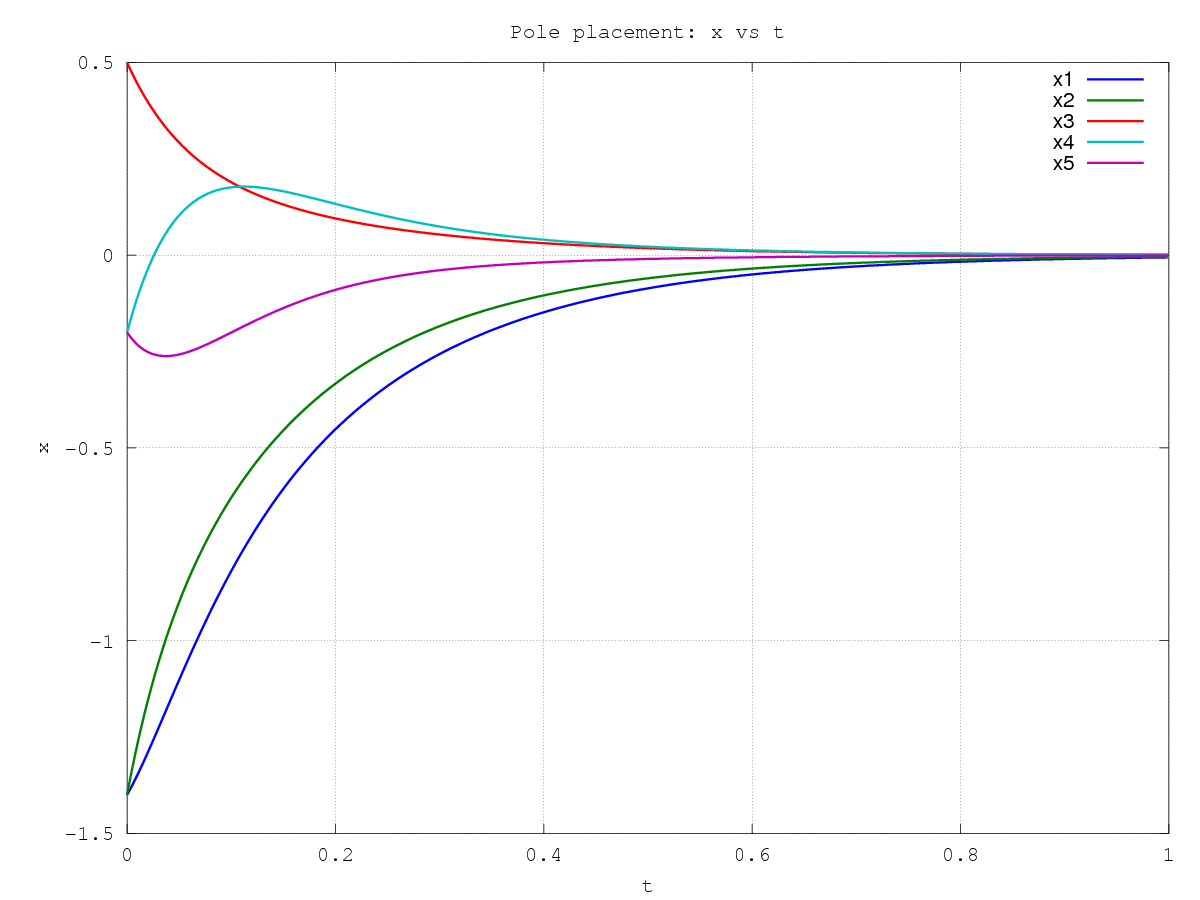
\includegraphics[scale=0.275]{figures/Question2x.png} 
	          \label{fig:Q2-x1}
              }
              \subfigure[$u(t)$ vs $t$]{
	          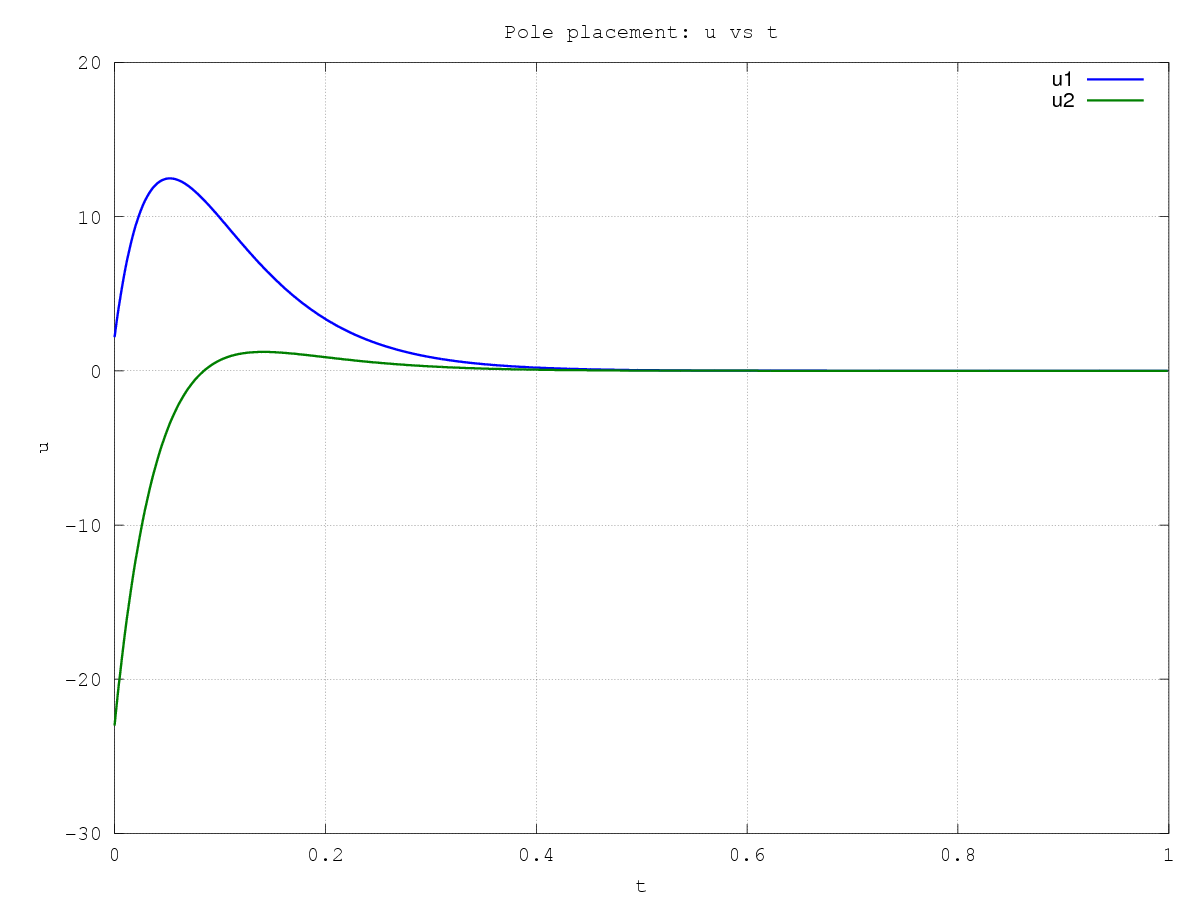
\includegraphics[scale=0.275]{figures/Question2u.png} 	
	          \label{fig:Q2-u1}
              }
            \caption{Results using pole placement}
            \label{fig:Q2-xu}
	\end{figure}

\subsection*{b}
Is the resulting $K$ the same as when you used optimal control in Question 1? If not, why not?
\subsection*{Solution}
The value of $K$ is not the same. In particular, the biggest difference is in the first row of $K_{pole}$, which is three times higher than the values of the first row of $K_{optimal}$. I think this is due to the fact that my optimal controller focuses on reduce the overall cost. In particular, since I made the cost of $u_{1}$ higher w.r.t $u_{2}$, it made the first row bigger, with more control effort.

I have to improve this answer. But by now, I will leave it here.

%%%%%%%%%%%%%%%%%%%%%%%%%%%%%%%%%%%%%%%%%
% Question 3
%%%%%%%%%%%%%%%%%%%%%%%%%%%%%%%%%%%%%%%%%
\section{}
Consider the block-diagram below. Assume that $r,u,y$ are all scalars and that $K$ has stabilized the closed-loop system. If the reference signal $r$ is constant, what should $K_{r}$ be such that $ \lim_{t \rightarrow \infty } y(t) = r$ ?

	\begin{figure}[H]
	\begin{center}
       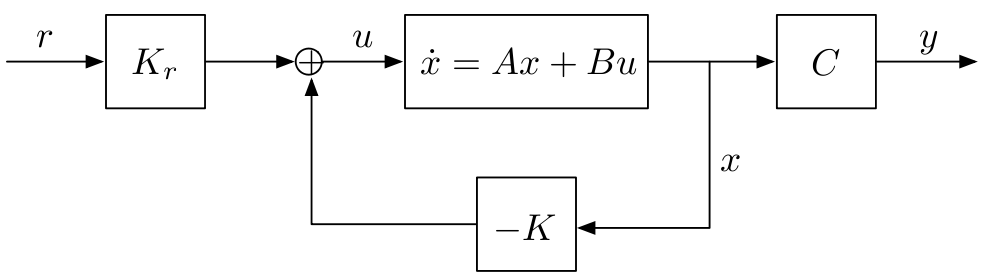
\includegraphics[scale=0.25]{figures/Question3.png} 
	   \label{fig:Question3}
	\caption{ x vs t}
	\end{center}
	\end{figure}
    
\subsection*{Solution}
Based on the system depicted above we have:

\[ \dot{x} = Ax + Bu \]
\[ u = K_{r}r - Kx \]
\[ y = Cx \]

Replacing $u$ in the differential equation:

\[ \dot{x} = Ax + BK_{r}r - BKx \]
\begin{equation} 
\dot{x} = (A-BK)x + BK_{r}r 
\label{Eq:Q3-dx}
\end{equation}

At infinite time ($t\rightarrow \infty$), $x$ is going to stabilize in $x_{ss}$:
\[ \lim_{t \rightarrow \infty} x = x_{ss} \]

Consequently, $\dot{x} = 0$:
\[ \lim_{t \rightarrow \infty}\dot{x} = 0 \]
\[ \lim_{t \rightarrow \infty} (A-BK)x + BK_{r}r = 0 \]

Replacing $x_{ss}$ in the limit:

\[ (A-BK)x_{ss} + BK_{r}r = 0 \]

\begin{equation} 
x_{ss} = -(A-BK)^{-1}BK_{r}r
\label{Eq:Q3-xss} 
\end{equation}

We are nearly done. Now, from the problem definition we have that:

\[ \lim_{t \rightarrow \infty } y(t) = r \]

but we know that $y = Cx$:

\[ \lim_{t \rightarrow \infty } Cx = r \]

Replacing $x_{t \rightarrow \infty } = x_{ss}$

\[Cx_{ss} = r\]

Replacing equation (\ref{Eq:Q3-xss}):

\[ -C(A-BK)^{-1}BK_{r}r = r \]

We can find $K_{r}$. Note that $-C(A-BK)^{-1}B$ is a scalar:
\begin{center}
\fbox{ $K_{r} = - \dfrac{1}{C(A-BK)^{-1}B}$ }
\end{center}

%%%%%%%%%%%%%%%%%%%%%%%%%%%%%%%%%%%%%%%%%
% Question 4
%%%%%%%%%%%%%%%%%%%%%%%%%%%%%%%%%%%%%%%%%
\section{}
Consider the scalar system

\[ \dot{x} = ax + bu \]
For this system, write a matlab program that finds the optimal $u$ that minimizes

\[ J(u) = \int^{1}_{0} (qx^{2}(t) + ru^{2}(t))dt + x^{2}(1)k \]

where $q,r,k > 0$. Plot and hand in your solution when $a=1$, $b=2$, $q=1$, $r=2$, $k=0.5$ and $x(0) = 1$

\subsection*{Solution}

\begin{center}
	\begin{figure}[H]
			  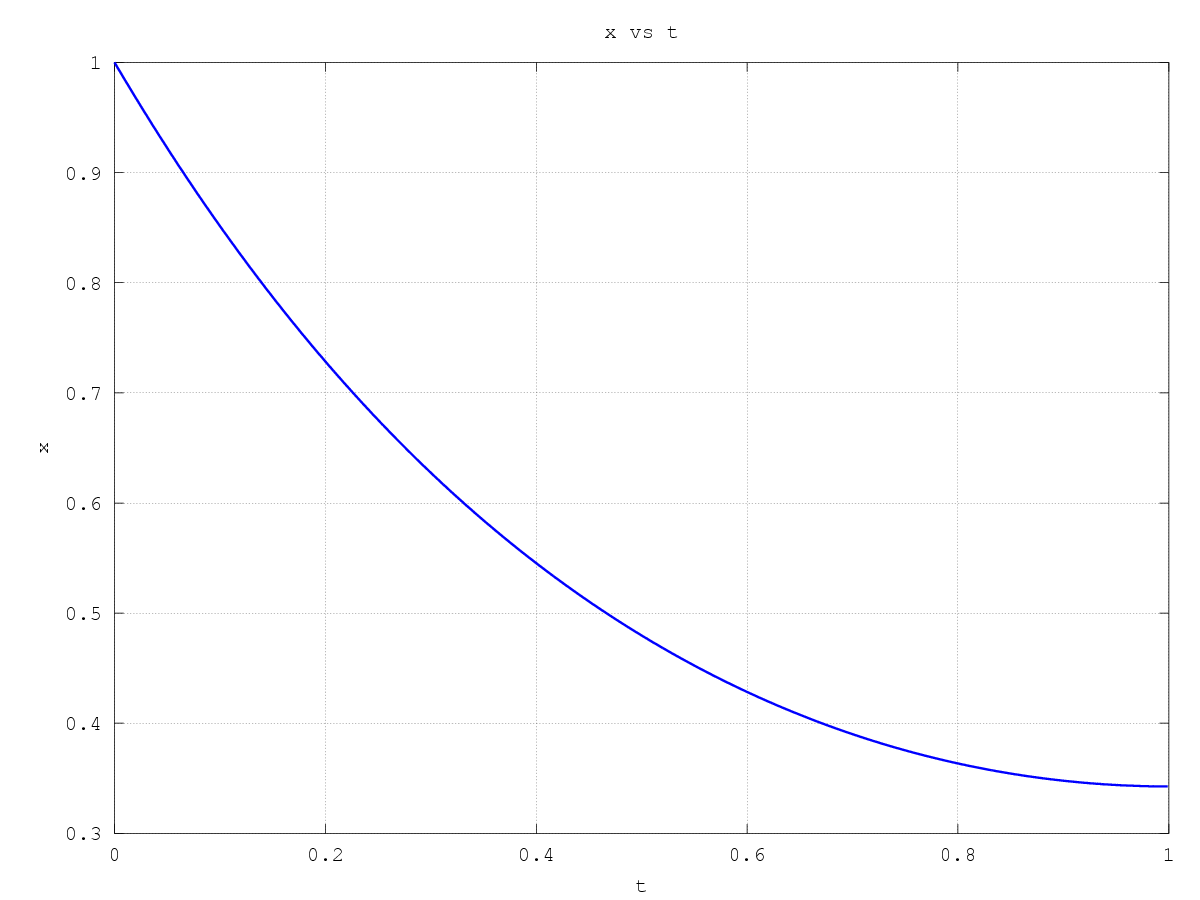
\includegraphics[scale=0.5]{figures/Question4X.png} 
	          \label{fig:Q4X}
	\caption{ x vs t}
	\end{figure}
	
	\begin{figure}[H]
			  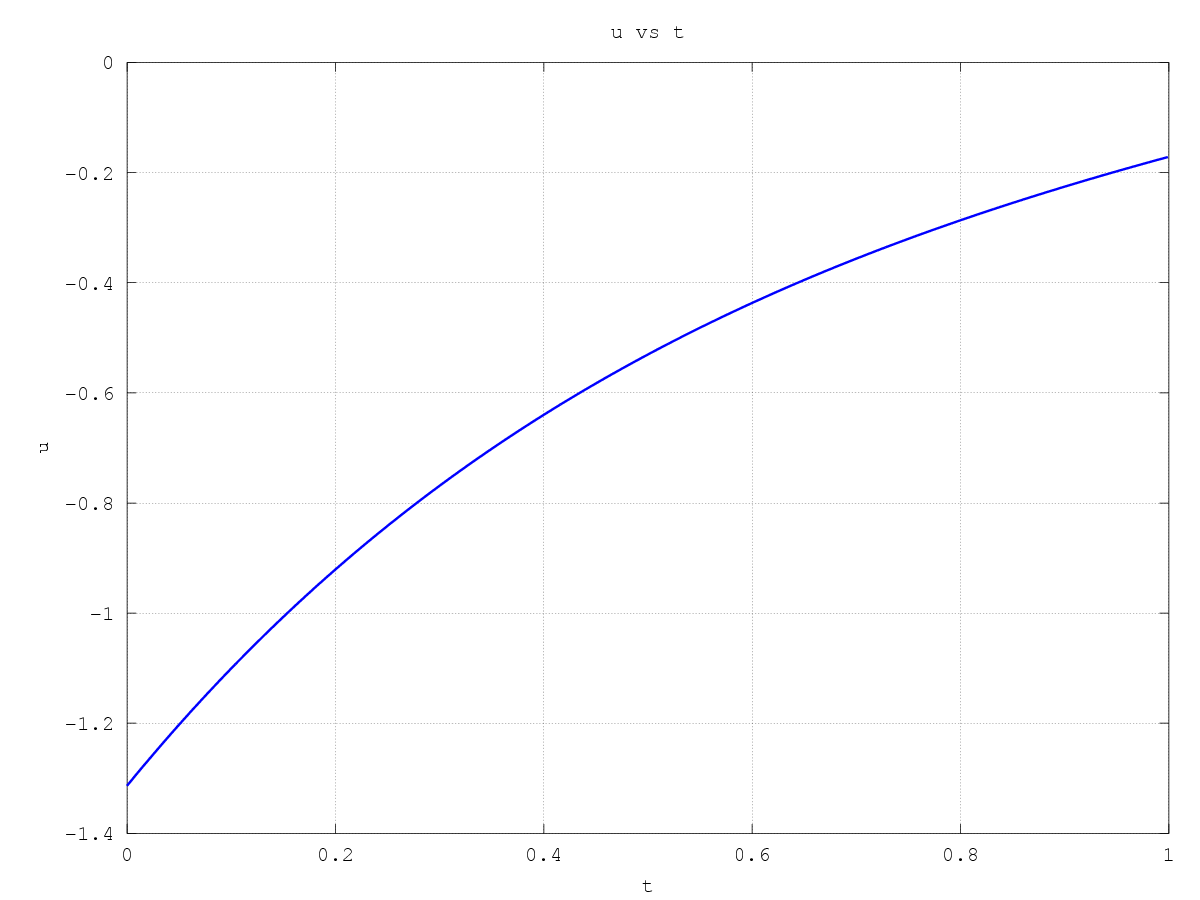
\includegraphics[scale=0.5]{figures/Question4U.png} 
	          \label{fig:Q4U}
	\caption{ u vs t}
	\end{figure}

	\begin{figure}[H]
			  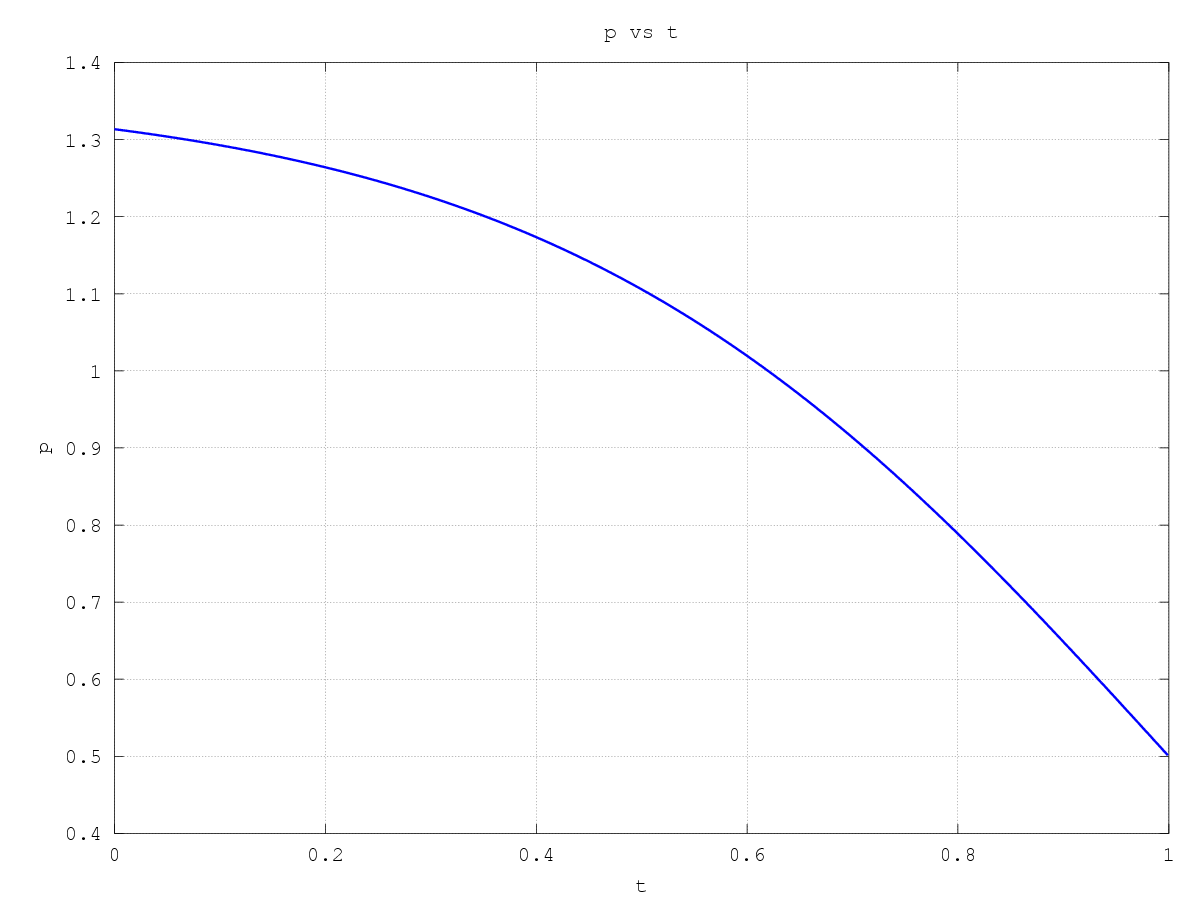
\includegraphics[scale=0.5]{figures/Question4P.png} 
	          \label{fig:Q4P}
	\caption{ p vs t}
	\end{figure}
\end{center}	

%%%%%%%%%%%%%%%%%%%%%%%%%%%%%%%%%%%%%%%%%
% Question 5
%%%%%%%%%%%%%%%%%%%%%%%%%%%%%%%%%%%%%%%%%
\section{}
Go to
\begin{center}
\texttt{http://www.cetl.gatech.edu/cios/digitalmeasures\_student.htm}
\end{center}

and check out the course survey for ECE6550-A. How many questions were there?

\subsection*{Solution}
I am resolving this way before the survey was opened so here my answer from last semester (when I took Optimal Control):
\medskip

There were 13 questions! (plus one verification question - something like {\em Did you take ECE 6553?} - and a comment box for 400 words (no profane language allowed, though)
\end{document}